\chapter{Partial Results}

\label{ch: Res}

The expected result of this work is a estimation software for parameters of Type-3 WTG's mathematical model \eqref{eq: Summary} in equation. To achieve this goal, the software will use the proposed hybrid estimation method of MVMO and TSM.

The measurements will be obtained from a small power system simulated on specific software, such as DIgSILENT or MATLAB. At first, the model proposed in \cite{Erlich2012} will be employed, but it can be further changed if needed. Also, other estimation methods, such as Particle Swarm Optimization, Differential Evolution or Kalman Filters, may be implemented for comparison purposes.

The hybrid approach for parameters estimation presented in this work is already implemented and have shown great results for different models. For learning and testing purposes, the proposed approach was used to estimate parameters of simpler systems, such as the spring-mass system, for testing purposes, but also in complex applications, such as load models. The results obtained from those systems are presented in the following subsections.

\section{Application of Hybrid Method on Spring-Mass System}

The spring-mass system is a simple physical model often used as example of dynamic systems. It is composed of an object of mass $m$ connected to a fixed point in space by a spring of stiffness constant $k$. When disturbed by an external force $u$, the object oscillates and its movement is described by \eqref{eq: SpringMass}, $x$ is the position of the object while $x_{1}$ and $x_{2}$ correspond to its speed and acceleration, respectively. The system output, parameter vector, input and initial conditions are presented on \eqref{eq: SMoutput}, \eqref{eq: SMp}, \eqref{eq: SMinput} and \eqref{eq: SMinitcond}, respectively.

\begin{equation}
	\begin{bmatrix}
		\dot{x_{1}} \\
		\dot{x_{2}}
	\end{bmatrix} = 
	\begin{bmatrix}
		0 & 1 \\
		\frac{k}{m} & 0
	\end{bmatrix}\cdot
	\begin{bmatrix}
		x_{1} \\
		x_{2}
	\end{bmatrix} -
	\begin{bmatrix}
		0 \\
		\frac{1}{m}
	\end{bmatrix}
	\cdot
	u
	\label{eq: SpringMass}
\end{equation}

\begin{equation}
	y = \begin{bmatrix}
		x_{1}, x_{2}
	\end{bmatrix}^ {T}
	\label{eq: SMoutput}
\end{equation}

\begin{equation}
	p = \begin{bmatrix}
		m, k
	\end{bmatrix}^ {T}
	\label{eq: SMp}
\end{equation}

\begin{equation}
	u = 1
	\label{eq: SMinput}
\end{equation}

\begin{equation}
	\begin{cases}
		x_{1}(0) = 0 \\
		x_{2}(0) = 0
	\end{cases}
	\label{eq: SMinitcond}
\end{equation}

The behaviour of the real system was obtained through simulation with parameters set at $m = 3\ kg$ and $k = 6\ N/m$. Three different estimation process were executed: TSM isolated, MVMO isolated and the hybrid approach proposed. The tolerance for all three estimations was set at $0.1$.

\subsection{Trajectory Sensitivity Results}

It took only 7 iterations to Trajectory Sensitivity Method estimate the parameters when the initial values were $m_{0} = 7\ kg$ and $k_{0} = 7\ N/m$. This shows how fast this method is when the initial values are in the neighbourhood of the real parameters. Figure \ref{fig: TS_conv} shows the error evolution during estimation suing TSM.

\begin{figure}[h]
	\caption{Error evolution of TSM with $m_{0} = 7\ kg$ and $k_{0} = 7\ N/m$}
	\begin{center}
		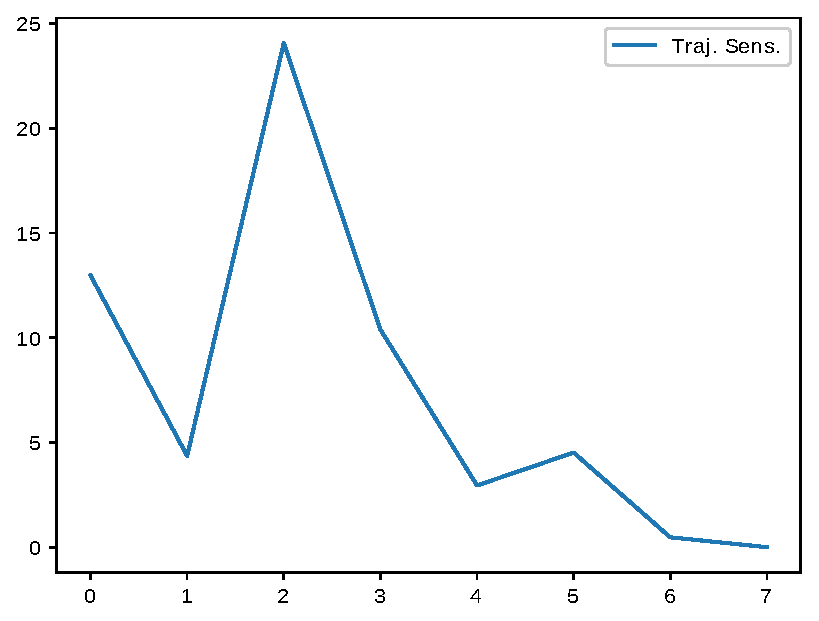
\includegraphics[scale=0.7]{Images/TS_conv.eps}
	\end{center}
	\label{fig: TS_conv}
\end{figure}

However, the convergence region of TSM is extremely limited, diverging from initial points far enough from the real values. The convergence region for the real values was obtained in \cite{Ecyo} and is shown in Figure \ref{fig: conv_reg}. For comparison, the MVMO and the hybrid approach converge for the entire search region displayed on the graph.

\begin{figure}[h]
	\caption{Convergence region of Trajectory Sensitivity Method}
	\begin{center}
		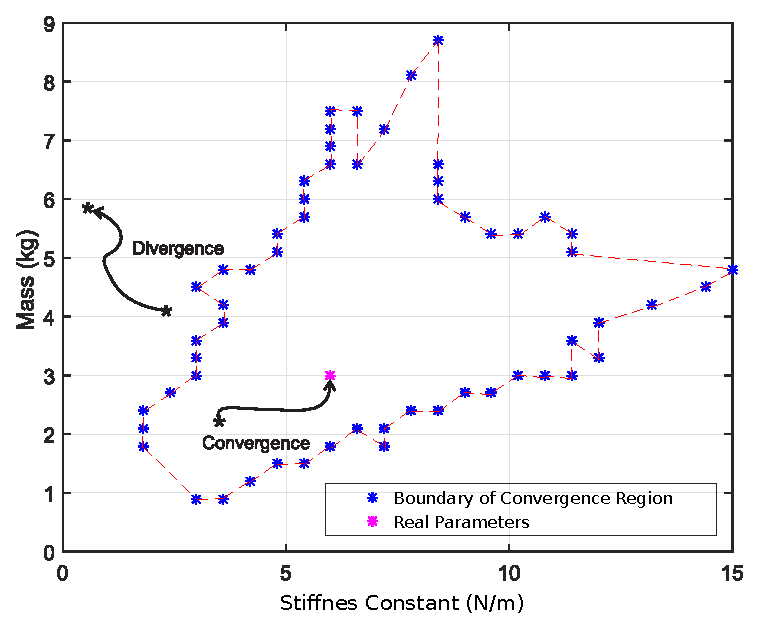
\includegraphics[scale=0.7]{Images/Conv_reg.eps}
	\end{center}
	\label{fig: conv_reg}
	\legend{Source: Adapted from \cite{Ecyo}}
\end{figure}

To illustrate the importance of good initial values, the parameters were reestimated using TSM, but now the initial values were set to be $m_{0} = 8\ kg$ and $k_{0} = 10\ N/m$. Notice that these values are not too far from the ones used in the previous estimation. The results, on the other hand, were extremely different. The method was not able to lower the error below $16.4$ and the parameters found were $m_{f} = 2.7\ kg$ and $k_{f} = 118.6\ N/m$. The error evolution for this estimation is depict in Figure \ref{fig: TS_nconv}.

\begin{figure}[h]
	\caption{Error evolution of TSM with $m_{0} = 8\ kg$ and $k_{0} = 10\ N/m$}
	\begin{center}
		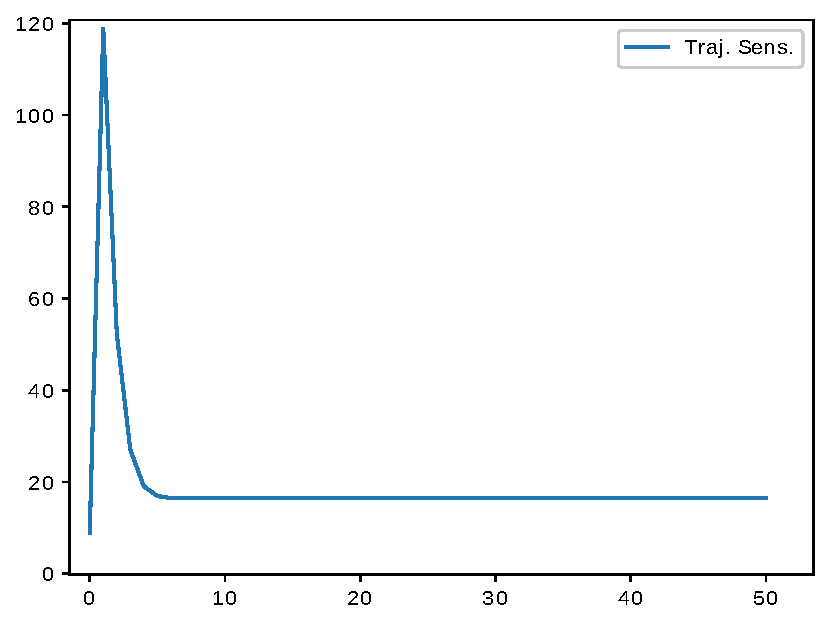
\includegraphics[scale=0.7]{Images/TS_nconv.eps}
	\end{center}
	\label{fig: TS_nconv}
\end{figure}

\subsection{MVMO Results}

The MVMO search region was defined as $0 \leq m \leq 9$ and $0 \leq k \leq 15$. The heuristic method converged after almost 10000 generations, as depicted in Figure \ref{fig: MVMO_conv}. This figure also shows how MVMO rapidly reduces error of estimation, but as the values approach the neighbourhood of the real values, it slows down.

\begin{figure}[h]
	\caption{Error evolution of MVMO}
	\begin{center}
		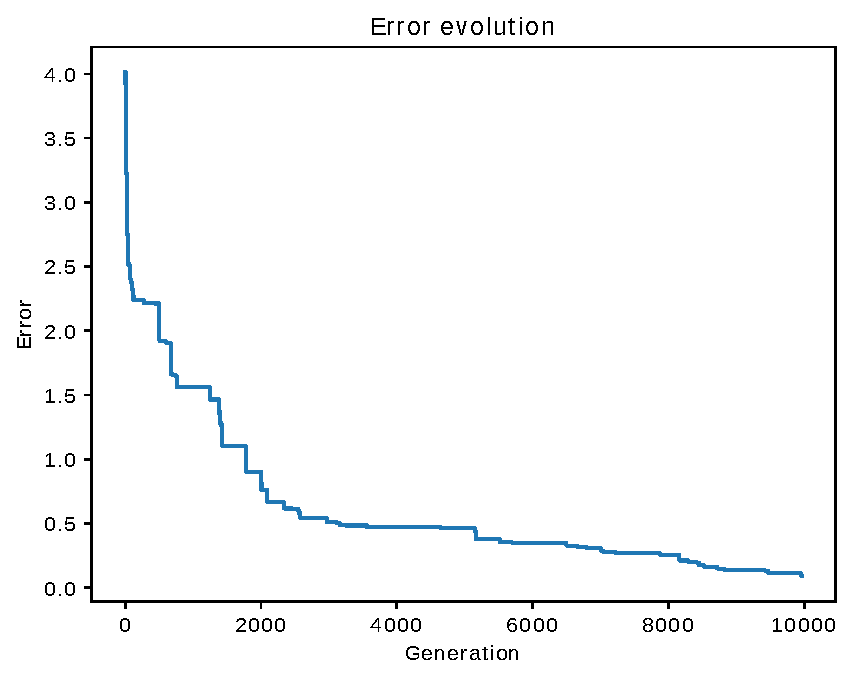
\includegraphics[scale=0.7]{Images/MVMO_conv.eps}
	\end{center}
	\label{fig: MVMO_conv}
\end{figure}

\subsection{Hybrid Approach Results}

By combining both methods, the hybrid approach benefits from the quick error reduction provided by MVMO and the fast convergence from TSM when inside convergence region. The error evolution obtained from this approach is depicted in Figure \ref{fig: Hybrid_conv}

\begin{figure}[h]
	\caption{Results of hybrid approach for spring-mass system}
	\begin{center}
		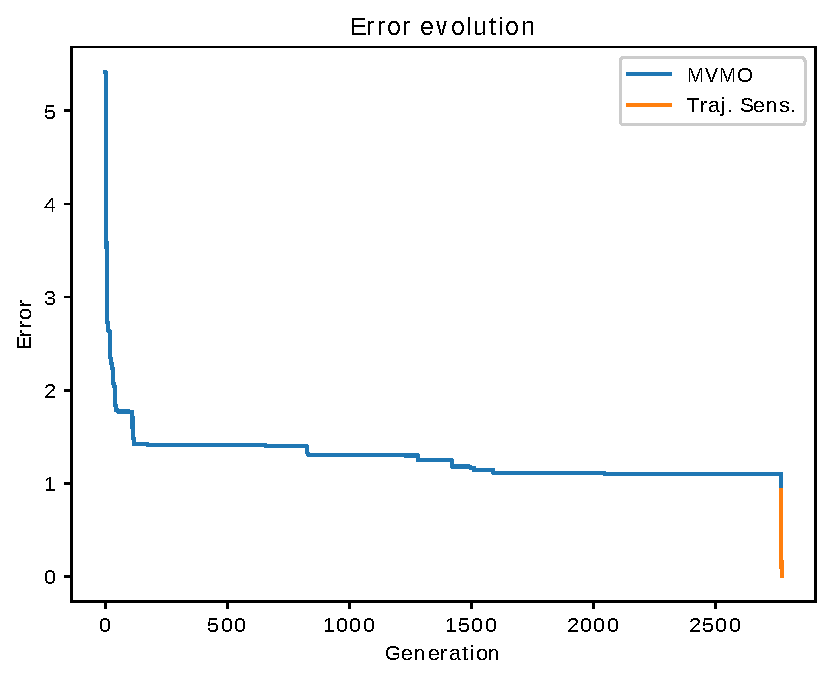
\includegraphics[scale=0.7]{Images/Hybrid_conv.eps}
	\end{center}
	\label{fig: Hybrid_conv}
\end{figure}

When compared to the methods alone, the hybrid approach converges faster than MVMO but slower than TSM, as shown in Table \ref{tab: SM}. Although all methods converged parameters with error level below the tolerance, TSM and the Hybrid approach provided a better behaviour than MVMO with final error close to $2.0\times 10^{-3}$.

\begin{table}[h]
	\caption{Comparison of approaches}
	\begin{center}
	\begin{tabular}{c|c|c}
		Approach & Time & Final Error \\
		\hline
		TSM  & $7 \ s$  & $2.76\times 10^{-3}$ \\
		MVMO  & $10 \ min$  & $89.33\times 10^{-3}$\\
		Hybrid  & $24 \ min$  & $1.54\times 10^{-3}$
	\end{tabular}
	\end{center}
	\label{tab: SM}
\end{table}

\section{Application of Hybrid Method on Z-IM Load Model}

The hybrid approach was also employed on parameter estimation of Z-IM load model and is subject of a paper presented by the author on the 2019 IEEE Canadian Conference on Electrical and Computer Engineering. This model is able to predict the behaviour of electrical loads during faults in the grid. It is described by the following equations:

\begin{equation}
    \begin{cases}
        \dot{E'} = \frac{1}{T_o}\left(\frac{X}{X'}E' + \frac{X - X'}{X'}V\cos\delta\right) \\
        \dot{\delta} = \omega - \omega_s - \frac{X - X'}{X'}.\frac{V\sin\delta}{T_o E'} \\
        \dot{\omega} = \frac{1}{M}\left(-\frac{VE'\sin\delta}{X'} - T_m\right)
    \end{cases}
    \label{eq: xZIM}
\end{equation}

Its outputs are the active and reactive power consumed by the load and are given by:

\begin{equation}
    \begin{cases}
        P = G_sV^2 - \left(\frac{VE'}{X'}\right)\sin\delta \\
        Q = B_sV^2 + \frac{V(V - E'\cos\delta)}{X'}
    \end{cases}
    \label{eq: yZIM}
\end{equation}

The Z-IM load model is much more complex than the spring-mass system, with 9 parameters to be estimated. The hybrid approach proposed was able to estimate the parameters of this system and the comparison between real and modeled behaviour with the parameters obtained can be seen in the Figure \ref{fig: ZIM}.

\begin{figure}[h]
	\caption{Result of parameter estimation for Z-IM Load Model}
	\begin{center}
		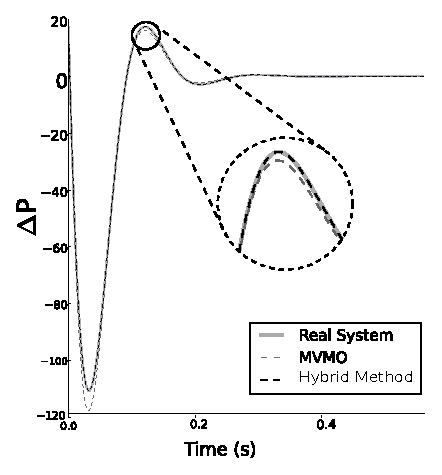
\includegraphics[scale=1]{Images/ZIM.eps}
	\end{center}
	\label{fig: ZIM}
	\legend{Source: \cite{Gomes2019}}
\end{figure}

\section{Ongoing Progress}

With the methods already implemented and tested, the focus is now on the DFIG model. The model has presented some results, but it is not as accurate as expected, requiring some studies about this topic. The implementation of other WTG models for comparison is also under study.

The simulation of wind turbine generators and power plants on specific software will be carried out on the next months. The GUI is under development and already has some features implemented using Python's library \textit{Tkinter}. A proposal to also develop features using \textit{Qt}, a different GUI tool package, is currently under consideration.